\subsection{Integrationsregeln}

\begin{Satz}{Satz von Fubini}{}
    Reduzierung von mehrdimensionalen Integralen auf eine Dimension. Sei $f: [a,b] \times [c, d]$ stetig, dann gilt
    \[ \int_a^b \int_c^d f(x, y) dx ~ dy = \int_c^d \int_a^b f(x, y) dy ~ dx = \int\displaylimits_{[a,b] \times [c, d]} f(x, y) dx ~ dy   \]

    Es sei der Quader $Q = [a_1,a_2] \times [a_2, b_2] \times \dots \times [a_n, b_n]$ mit $f \in C^0(Q)$ gegeben. Dann gilt

    \[
        \int_Q f(x) d\mu(x) = \int_{a_1}^{b_1} dx_1 \int_{a_2}^{b_2} dx_2 \dots \int_{a_n}^{b_n} dx_n f(x_1, x_2,...,x_n)
    \]
    
    \textbf{Die Integrationsreihenfolge darf vertauscht werden.}
\end{Satz}

Alternative Schreibweise von $dx ~ dy$: $\mu(x, y)$, $\mu(x+y)$.

\subsection{Normalbereiche in $\R^2$}

\begin{Definition}{Normalbereiche in $\R^2$}{}

Sei $\Omega$ eine beschränkte Teilmenge von $\R^2$. $\Omega$ heisst \textbf{y-Normalbereich}, falls sich $\Omega$ wie folgt darstellen lässt:

\[
    \Omega = \{(x, y) \in \R^2 \mid a \leq x \leq b, f(x) \leq y \leq g(x)\}
\]

wobei $f$, $g$ stetige Funktionen der Variable $x$ sind. Die Rolle von $x$ und $y$ darf vertauscht werden (es existiert also auch ein $x$-Normalbereich).

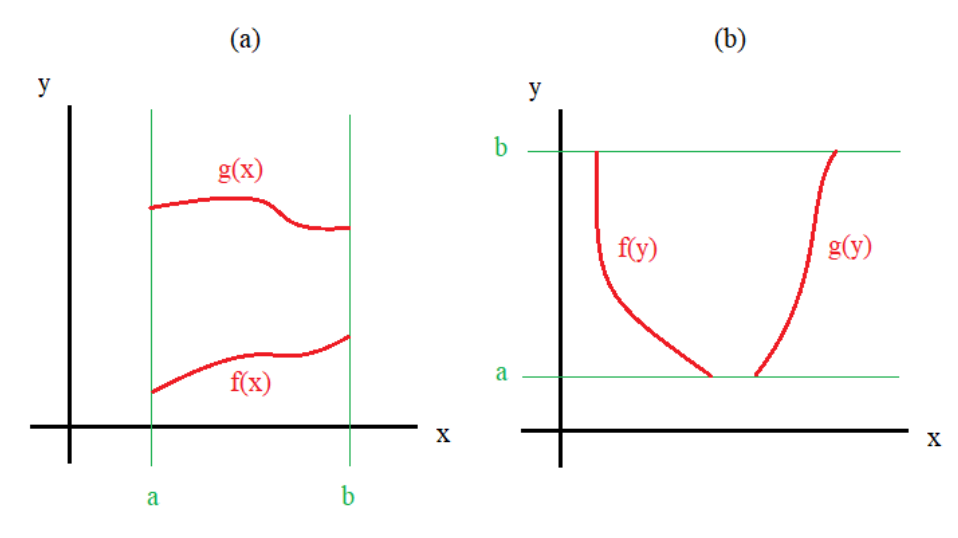
\includegraphics[width=10cm]{images/normalbereich}

(a): y-Normalbereich, (b): x-Normalbereich

\end{Definition}
\begin{Satz}{Integration auf Normalbereichen}{}

Sei \[\Omega = \{(x, y) \in \R^2 \mid a \leq x \leq b, f(x) \leq y \leq g(x)\}\] ein \textbf{y-Normalbereich} mit stetigen Funktionen $f$, $g$ und sei die zu integrierende Funktion $F \in C^0(\Omega)$, dann gilt:

\[
    \int_{\Omega} F d\mu = \int_a^b dx \int_{f(x)}^{g(x)} dy F(x, y)
\]

Das innere Integral wird zuerst ausgewertet.
\end{Satz}

\begin{Rezept}{Integrieren über Normalbereichen}{}
Am folgenden Beispiel:
\[ \int_D f(x, y) ~ dx dy ~~ \text{ wobei } ~~ D = \R^2 \cap \{(x, y) ~ | ~ y \geq 0 ~ \wedge ~ x-y+1\geq 0 ~ \wedge ~ x+2y-4 \leq 0\}\]
\begin{enumerate}
\item {
Es hilft, sich den Normalbereich visuell vorzustellen, um die Grenzen
zu finden. Bedingungen nutzen:
\[ y \geq 0 ~ \wedge (y-1 \leq x \leq 4-2y) \]
Damit $x$ nicht leer ist, muss $y-1 \leq 4-2y$ sein, resp. $y \leq \frac{5}{3}$ 
}
\item {
Für das äussere Integral sind die Integrationsgrenzen nun fest vorgegeben. Die inneren Grenzen
werden abhängig von der äusseren Variable gewählt:

\[ \int_D f(x,y) ~ dx dy = \int_0^{\frac{5}{3}} \int_{y-1}^{4-2y} f(x,y) ~ dx dy \]

}
\end{enumerate}
\end{Rezept}

\begin{Rezept}{Area($D$) - Vol($D$) - Volumen eines Normalbereichs in $\R^n$}{}
Analog zum Integrieren über Normalbereich:
\[ \text{Vol}(D) = \int_D 1 ~ dX = \underbrace{\int \!\! \int \ldots \int}_{n} 1 ~ dx_1 \ldots dx_{n-1} dx_n,
  ~~~~ D \subset \R^n\]
\end{Rezept}



\begin{Satz}{Substitutionsregeln in einer Dimension}{}
    Sei $f$ eine Riemann-integrierbare Funktion. Für die Berechnung des Integrals
    \[
        \int_a^b f(x) dx
    \]
    führt die Substitution $x \to g(u)$ zu $dx = g'(u)du$ und damit wird das Integral
    \[
        \int_a^b f(x) dx = \int_{g^{-1}(a)}^{g^{-1}(b)} f(g(u)) g'(u) du
    \]
    Das heisst wir haben das Integrationselement $dx$ durch $g'(u)du$ ersetzt und die Grenzen entsprechend angepasst.
\end{Satz}

\begin{Satz}{Substitutionsregeln in $n$ Dimensionen}{}
    Sei $f$ eine Riemann-integrierbare Funktion auf dem Gebit $\Omega \subset \R^n$ und die Koordinatentransformation (Substitution)
    \[
    (x_1,\hdots,x_n) = \Phi(u_1, \hdots,  u_n)
    \]
    oder in Komponenten
    \[
        \vek{x_1}{\vdots}{x_n}
        = \Phi(u)
        = \vek{g_1(u_1,\hdots,u_n)}{\vdots}{g_n(u_1,\hdots,u_n)}
    \]
    ist ein $C^1$-Diffeomorphismus. Dann gilt
    \[
        \int_\Omega f(x_1, \hdots, x_n)dx_1\hdots dx_1 = \int_{\widetilde{\Omega}} f(g_1(u), \hdots, g_n(u)) \cdot |\det d \Phi|\ du_1\hdots du_n
    \]
    wobei das Gebiet $\widetilde{\Omega} = \Phi^{-1}(\Omega)$ ist. $|\det d\Phi|$ ist die \textbf{Funktionaldeterminante} (Jakobi-Determinante).
\end{Satz}

\begin{Rechenregeln}{Wichtige Koordinatentransformationen und Funktionaldeterminanten}{}
    \begin{itemize}
       \item Polarkoordinaten in $\R^2$ \begin{alignat*}{4}
            x &= r \cos \varphi\quad &&0 \leq r < \infty\quad &&&dxdy = r \cdot drd\varphi\\
            y &= r \sin \varphi\quad &&0 \leq \varphi < 2\pi\quad
        \end{alignat*}
        \item Elliptische Koordinaten $\R^2$ \begin{alignat*}{4}
            x &= r \cdot  a \cos \varphi\quad &&0 \leq r < \infty\quad &&&dxdy = a \cdot b \cdot  r \cdot drd\varphi\\
            y &= r \cdot b \sin \varphi\quad &&0 \leq \varphi < 2\pi\quad
        \end{alignat*}
        \item Zylinderkoordinaten $\R^3$ \begin{alignat*}{4}
            x &= r \cdot  a \cos \varphi\quad &&0 \leq r < \infty\quad &&&dxdydz = r \cdot drd\varphi dz\\
            y &= r \cdot b \sin \varphi\quad &&0 \leq \varphi < 2\pi\quad\\
            z &= z\quad &&\-\infty \leq z < \infty\quad
        \end{alignat*}
        \item Kugelkoordinaten $\R^3$ \begin{alignat*}{4}
            x &= r \cdot \sin \theta \cos \varphi \quad &&0 \leq r < \infty\quad &&&dxdydz = r^2 \sin \theta \cdot drd\theta d\varphi\\
            y &= r \cdot \sin \theta \sin \varphi \quad && 0 \leq \theta < \pi\quad\\
            z &= r \cos \theta \quad &&0 \leq \varphi < 2\pi\quad\quad
        \end{alignat*}
   \end{itemize}
\end{Rechenregeln}

\begin{Satz}{Satz von Green in der Ebene}{}
	\textbf{TODO}	
\end{Satz}

\begin{Rezept}{Flächen berechnen mit Satz von Green}{}
	\textbf{TODO}	
\end{Rezept}

\begin{Satz}{Masse und Schwerpunkt}{}
	\textbf{TODO}	
\end{Satz}

\begin{Satz}{Satz von Gauss}{}
	\textbf{TODO}	
\end{Satz}

\begin{Satz}{Pappus}{}
	\textbf{TODO}	
\end{Satz}

\begin{Satz}{Satz von Stokes}{}
	\textbf{TODO}	
\end{Satz}
